\documentclass[conference]{IEEEtran}
\IEEEoverridecommandlockouts
% The preceding line is only needed to identify funding in the first footnote. If that is unneeded, please comment it out.
\usepackage{cite}
\usepackage{amsmath,amssymb,amsfonts}
\usepackage{algorithm}
\usepackage{algpseudocode}
\usepackage{graphicx}
\usepackage{textcomp}
\usepackage{xcolor}
\algrenewcommand\algorithmicrequire{\textbf{Input:}}
\algrenewcommand\algorithmicensure{\textbf{Output:}}
\def\BibTeX{{\rm B\kern-.05em{\sc i\kern-.025em b}\kern-.08em
    T\kern-.1667em\lower.7ex\hbox{E}\kern-.125emX}}
\begin{document}

\title{A perusal of the 2018 Russian Presidential Election - The triumph of Vladimir Putin\\}

\author{\IEEEauthorblockN{Anurag Dutta}
\IEEEauthorblockA{\textit{Undergraduate, Computer Science and Engineering} \\
\textit{Government College of Engineering and Textile Technology, Serampore}\\
Calcutta, India \\
anuragdutta.research@gmail.com}
}

\maketitle

\begin{abstract}
The 2018 Russo - Presidential Election was the 3’rd consecutive triumph for President Putin in the Presidential Elections. Well! he is quite well known for his courage and love for Russia and its alliances, which ended him being elected as the President for a tenure of 6 Years, by the Russian citizens for the 3’rd time in the sequel. In this work, we would be scrutinizing the validity of the 2018 Russian Presidential Election, or rather prove the validity of the result, as an exercise, subjecting to the famous Benford’s Law, put through improvisations on the strata of Machine Learning Techniques. To clarify, the data, used for this purpose is available, free of copyright, as per CC0 1.0 Universal (CC0 1.0). \\
\end{abstract}

\begin{IEEEkeywords}
Fraud Detection, Benford’s law, Zipf’s law, 2018 Russo - Presidential Election, Statistical Machine Learning
\end{IEEEkeywords}

\section{Introduction}
Fraud, the word itself means any action, method, or scheme that does not comply with the laws laid down for the children of Mother Earth. Since the first scam around 300 BC, not much has changed to this day. As time passed, societies grew, colonization took place, and the economy boomed and waned, but the inner urges of human beings remained the same. To this day, fraud happens every day. Scammers are very clever, but the laws of nature cannot be ruled out. However, the difficulty of reaching definitive climate assessments or election results based on direct and indirect observations precludes objective and actionable monitoring, as Russia did in 2008. , that the regime can build inexplicable and formidable administrative barriers to shut them down. Alternatively, as happened in Ukraine in 2004, both sides of the dispute can deploy their own observer cadres to allege or deny indirect or direct fraud. Moreover, Benford's Law and Zipf's Law can be combined to produce robust and conclusive results for most types of fraud that occur in everyday life, including income tax fraud, credit card fraud, GDP fraud, and election fraud. increase. Benford's law (Frank Benford 1938), also known as the first-digit law or the anomalous digit law, is his first-digit rule for random, large, and diverse datasets. Logarithmic probability distribution function. The first significant digit of a number is the first non-zero leftmost digit, such as 6 for 6897, 9 for 99, 7 for 0.007895, and so on. According to the proposed Benford's Law, in a defined dataset, the probability of a particular digit being prevalent as a starting number decreases logarithmically as the value of the digit increases from 1 to 9. increase. The expected probability values are summarized in the table below
\begin{table}[htbp]
\caption{Probability of occurrence of digits using Benford’s law}
\begin{center}
\begin{tabular}{|c|c|}
\hline
\textbf{\textit{Digit}} & \textbf{\textit{Probability}} \\
\hline
1       & 0.301029 \\
\hline
2      & 0.176091 \\
\hline
3     & 0.124938 \\
\hline
4    & 0.096910 \\
\hline
5   & 0.079181 \\
\hline
6  & 0.066946 \\
\hline
7 & 0.057991 \\
\hline
8 & 0.051152 \\
\hline
9 & 0.045757 \\
\hline
\end{tabular}
\label{tab1}
\end{center}
\end{table}
Zipf's law is a pragmatic law developed using mathematical and probability statistics, which refers to the fact that for certain pieces of information studied in the physical sciences and math, the rank frequency distribution has an inverse relationship between them. The Zipfian distribution is a discrete power law probability distribution. It deals with the zeta distribution, it deals with similar but not identical types of data sets. Zipf's law was originally formulated for linguistics to study the irregular occurrences of words, showing that, given a corpus or dataset of occurrences of natural languages, the frequency of occurrence of a word is inversely proportional to its rank in the frequency table. Thus, the most frequent word will appear twice as often as the second most frequent, three times as often as the third, and so on. For example, in the Brown Corpus of American English text, the word "the" is the most frequent word and alone accounts for nearly 7.0\% of the word's total occurrences. This law was created after the American linguist George Kingsley Zipf (1902–1950). Although he is not the only one who invented this logic or rather the law. The French stenographer Jean-Baptiste Estoup (1868–1950) also noticed this pattern before Zipf mentioned it. Furthermore, it was also noticed by the German physicist Felix Auerbach (1856-1933) in 1913. These laws have been enacted on many frauds and have been successful in detecting fraud in many cases. Some other aspects where Benford law has been used quite often are checking election results, checking someone's income tax details, credit card transactions, etc. 
\section{Recent Works}
[1] Mark J. Nigrini, has used Benford's method in the field of fraud detection and forensic analysis. His analysis involves various advanced theoretical works on Benford Law and the various legal processes surrounding fraud allegations. Mark J. Nigrini is the author of Forensics Analytics (Wiley Publications), which describes tests, i.e. Benford's Law, for detecting fraud, errors, estimates, and biases in monetary and election information. He has been praised by the national media, including the "Wall Street Journal" and has published numerous articles on Benford's law. [2] Work by Arno Berger and Theodore P. Hill talked about the randomness of Benford's Law, that it should only be applied to some specific data sets. to ensure an accurate and precise result, otherwise this rule has more disadvantages than advantages. [3] Hill, Theodore's research paper attempted to explain the many possibilities of using Benford's law in areas such as computer design, mathematical modeling, and discovery. fraud in accounting data. [4] Research by Innocent Mbona, and Jan H. P. Eloff focuses on finding alternatives to malicious social media programs. The study found that feature selection follows Benford's law on the average human dataset, while the equivalent option violates Benford's law on malicious bot datasets. This study demonstrates that the choices recognized by the Benford law field are consistent and therefore identical with the information provided by the PCA and follow the random forest technique on the equivalent dataset. [5] Aleksandar Tošić, Jernej Vičič: His research focuses on the application of Benford's law to scientific cooperative networks. The paper proposes a unique methodology to assess the maturity of the research system. The paper examines the anomalies found among the diverse and disparate research fields in  Slovenia. [6] A research paper by Joanne Horton, Dhanya Krishna Kumar, and Anthony Wood titled discussed the potential of Benford's law in detecting the validity of underlying data used in various academic and research papers. [7] Neumann and Peter G have shown a basis for the statistical metallographic use of Zipf's law, which opens us up to an excellent way to suggest the applicability of this law. in various statistical fields. [8] Piantadosi, Steven's research paper shows many possible uses for Zipf's Law, from areas like statistical linguistics to fraud detection. Piantadosi and Steven worked to verify Zipf's law by taking a dataset as a data store of different words studying the occurrences of some specific frequent words and then classifying them to apply the definition: of Zipf law. [9] Belevitch V's research paper was one of the first articles written on Zipf's law and its applications. This article discusses different perspectives of statistical methods that can be applied to Zipf's law. The core of this paper focuses on the irregular distribution of some words that occur more often than others and thus investigates its frequency distribution using different statistical methods. [10] Jing Wei, Jianjun Zhang, and Bofeng’s Research paper by Cai, Ke Wang, Sen Liang, and Yuhuan Geng processed data sets of CO2 emissions from different cities in China and verify them based on testing of experimental data. The proposal offers a modified model to explore the development of Chinese cities. [11] A research paper by Qiuping A. Wang proposed a new method to derive the Zipf-Pareto law using the rule of least effort. An approach that combines the higher computing power and non-additive probabilities of an efficient thermodynamic engine leads to the deduction of the Zipf-Pareto law. [12] A research paper by Michael E. Adel suggested that ideas related to business information could be inferred from patent topography using Pareto-analysis. 
\section{Benford's Law}
Benford's Law is an observation-based law discovered in the  1800s, when a Canadian-American astronomer Simon Newcomb observed that in his diary, the first few pages, especially those that start with `1` are in worse condition than the following pages. This observation created a stream of thoughts in his head, which then formed a formula. Newcomb proposed a law stating that  the probability of being the first digit of a number for a single number $\lambda$ is equal to $log(\lambda\ +\ 1)\ -\ log(\lambda)$. In the late 1900s, the phenomenon was noted again  by a physicist, Frank Benford, who applied the then known formula to many data sets and to his surprise was virtually all data sets show correlation with words. The total number of sightings used by Benford in his paper was close to 20,000, which was indeed a huge number to deal with at the time. Anyways, later Benford got recognition for it. In short, Benford's Law states (or rather observes) that many processes or measures give rise to numbers (e.g., return on investment, population of major cities, addresses of locations, business sales, tower and building heights) setting up denominators can seem counterintuitive, where lower numbers are more common than higher numbers. Mathematical Formula of Benford's Law is $\pi(\delta)\ =\ {log}_{10}{\left(1\ +\ \frac{1}{\delta}\right)}$, where, $\pi(\delta)$ is the Probability of Occurrence of the digit $\delta$ as the first digit $\ni\forall\ 1\ \le\ \delta\ \le\ 9$. 
\begin{figure}[htbp]
\centerline{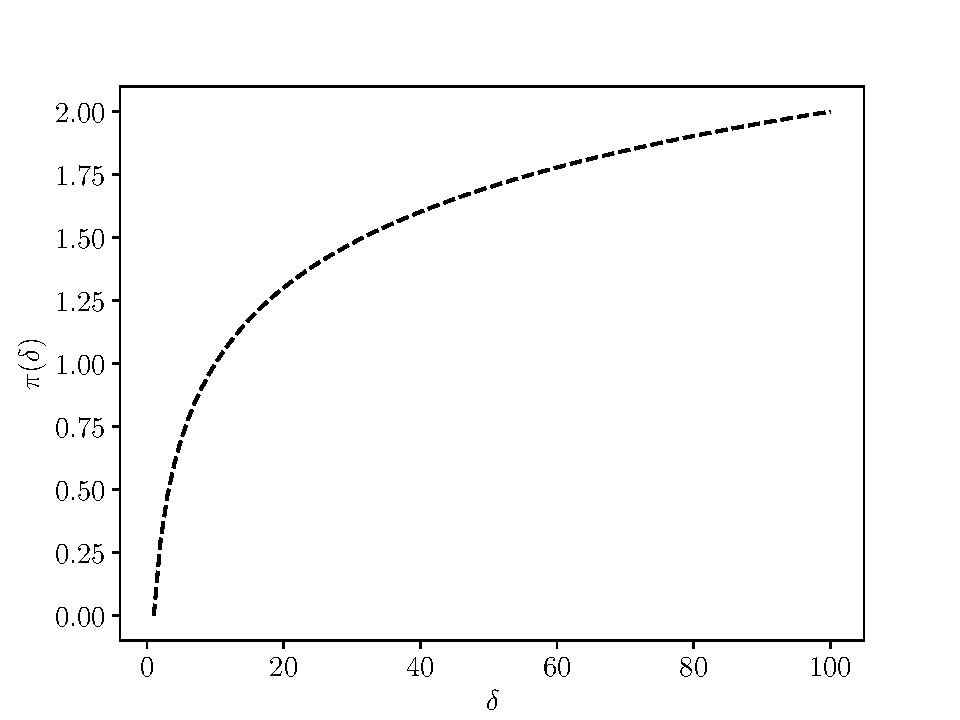
\includegraphics[width = \linewidth]{1}}
\label{fig1}
\caption{Graph for Benford’s law where $x$-axis denotes the first digits and $y$-axis denotes their corresponding probabilities.}
\end{figure}
Figure 1 shows Graph for Benford’s law where $x$-axis denotes the first digits and $y$-axis denotes their corresponding probabilities. In the plot given above, $\pi(\delta)$ was confined on the y – axes while $\delta$ on the x – axes. The above formula only works when the digit is only  the first digit, although another formula has been created that tells us about the probability of the $\zeta$’th digit. Coherently, the value of $\pi\left(\delta\right)$ could be delineated as
\begin{equation*}
\pi=\left\{\begin{matrix}{log}_{10}{\left(1\ +\ \frac{1}{\delta}\right)}&\ni\ \forall\ 1\ \le\ \delta\ \le\ 9\\\sum_{\kappa={10}^{\zeta-2}}^{\kappa={10}^{\zeta-1}-1}{log}_{10}{\left(1+\frac{1}{10\kappa+\delta}\right)}&\ni\ \forall\ 0\ \le\ \delta\ \le\ 9\\\end{matrix}\right.
\end{equation*}
\section{Zipf's Law}
George Kingsley Zipf, an American linguist and philologist who has studied statistical occurrences, the name Zipf's Law, proposed in 1935 that some words are repeated frequently while many or most are rarely used. This is the main driving force for Zipf's Law. In a nutshell, Zipf's Law prescribes (or rather observations) the various  data collections used to study the physical sciences. In theory and in scientific society, the frequency-rank distribution exists in an inverse relationship. Zipf's law was originally formulated in perceptual linguistics, according to which, for any  natural language corpus, some words appear very frequently while others appear quite frequently. rare. Now, if a word appears in the histogram, its occurrence frequency  will be inversely proportional to the rank the word earns on the histogram. So, the most frequent word will appear twice as often as the second, three times as often as the third, and so on, but this rule is not limited to linguistics, it is also can be applied to arithmetic as well. Given a data set  sorted in ascending order, in such a case the frequency multiplied by the rank would be a constant. Mathematically, $f_\varsigma\times\varsigma\ =\ \psi$, where, $f_\varsigma$ = Frequency of data with rank $\varsigma$, and $\psi$ being a constant. 
\section{2018 Russo - Presidential Election}
The 2018 Russo - Presidential Election was the 7’th Presidential Election on the Russian Soil. It was held on the 18’th of March ’18. Figure 2 shows the Election Mascot.
\begin{figure}[htbp]
\centerline{
\includegraphics[width = \linewidth]{2}}
\label{fig2}
\caption{Election Mascot for the 2018 Russo - Presidential Election}
\end{figure}
It started in 2017, when incumbent Vladimir Putin was running for re-election. He announced his intention to do so on December 6, 2017, and he was widely expected to win. This came after months of speculation in late 2017 that Putin would run for the next term the president wanted, despite widespread expectations that he would run for the next term, made evasive remarks, including that he had  not  yet decided whether "He is resigning", he said, "I will consider running for public office" Various sources predicted that Putin would run as an independent to gain more popular support, and although he could  have been nominated by the United Russia Party as in 2012, Putin as an independent, chose to run. 67.5\% of registered voters in Russia took part in the election. Vladimir Putin was well known and praised during his KGB days for his love and devotion to Russian soil, which can still be seen today. And as expectations would seem to, Putin got re elected for the 3’rd Time in Sequel, for a tenure of 6 years. Now, rumours were murmured about the fraudulency of the result. In this work, we would like to get an alpha out of the cumbersome. 
\begin{figure}[htbp]
\centerline{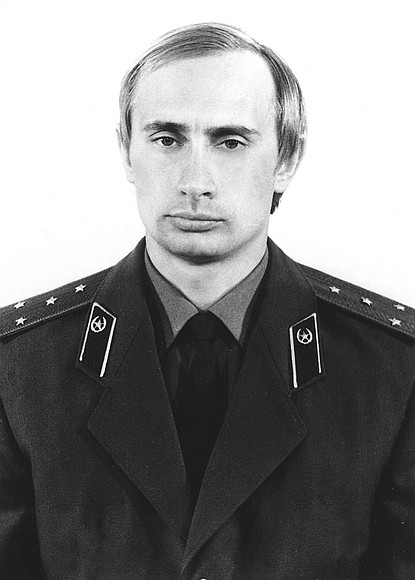
\includegraphics[width = \linewidth]{3}}
\label{fig3}
\caption{Vladimir Putin during his days in the \textit{Komitet Gosudarstvennoy Bezopasnosti}}
\end{figure}
\end{document}
